\section{Real-data application: NGSIM vehicle trajectories}
\label{sec:real}

\subsection{Data, observed outcomes and evaluation protocol}
We use camera-derived longitudinal positions from
US-101 and I-80 in the U.S. Federal Highway Administration
NGSIM dataset \citep{fhwa2016}. The position
\texttt{Local\_Y} is converted from feet to meters.
The observations are sampled at 10\,Hz. Episode
extraction requires consecutive 100-ms time steps
and uses historical quality-control rules, with
future evaluation data excluded from model fitting.
Vehicle identifiers can recur across capture periods.

Our principal real-data study evaluates 200
preselected episodes, 100 per site, associated
with 113 distinct (site, numerical vehicle-ID)
pairs across five coarse capture-time blocks.
Each episode uses a single chronological origin
with 80 previous position measurements (8\,s)
and holds out 5, 10 or 20 subsequent frames
for 0.5-, 1- and 2-second evaluation.
All reported comparisons use the same
episode and horizon targets. The empirical
outcome is future \emph{recorded position},
not the unobserved noise-free path or
independently measured physical jerk.

The selection is a convenience sample from
bounded official data queries, not a random
sample of all vehicle motions. Correlation
within recording scenes, shared time blocks,
repeated reported IDs and forecast horizons
rules out naive independent-episode
population significance tests. Complete
source-page hashes, episode catalogs,
selected positions and error records are
preserved in Experiment004; Experiment006
reuses the exact same real episodes.

\subsection{Comparison with smoothing splines,
Savitzky--Golay and polynomial trends}
\begin{table*}[t]
\centering
\caption{Main real-data comparison: pooled future
\emph{recorded-position} RMSE (meters) over
200 NGSIM episodes. GCV or conditional
profile Gaussian likelihood selects
smoothing using training observations
only; the three-point and local-25 rules
are separate continuations of a fitted
PLS trend. All rows have 200 valid episodes
at each horizon. Bold highlights the
smallest pooled RMSE, not statistical
superiority over a population.}
\label{tab:ngsim-main}
\begin{tabular}{lccc}
\toprule
Smoother and continuation & 0.5\,s & 1\,s & 2\,s\\
\midrule
Natural cubic smoothing spline, GCV + quadratic Taylor
 & \textbf{0.1354} & \textbf{0.3480} & \textbf{0.8787}\\
PLS $d=3$, $\mu=0$, profile ML, three-point
 & 0.1433 & 0.5124 & 1.8686\\
PLS $d=3$, $\mu=0$, GCV, three-point
 & 0.1453 & 0.5166 & 1.8805\\
PLS $d=3$, sample $\widehat\mu$, profile ML, three-point
 & 0.1457 & 0.5310 & 2.0142\\
PLS $d=3$, sample $\widehat\mu$, profile ML, local-25
 & 0.3166 & 0.5764 & 1.3535\\
Raw local quadratic polynomial, 25 points
 & 0.3406 & 0.6184 & 1.3447\\
Savitzky--Golay, quadratic Taylor
 & 0.3547 & 0.8506 & 2.4106\\
\bottomrule
\end{tabular}
\end{table*}

Table~\ref{tab:ngsim-main} shows that
the GCV-selected smoothing spline attains
the lowest pooled forecast RMSE at all three
horizons. At half a second, zero-reference
PLS with profile likelihood and three-point
continuation is relatively close
(0.1433\,m versus 0.1354\,m), but its
error increases sharply with the horizon.
The local-25 continuation may reduce
longer-horizon PLS error at the cost
of worse short-horizon behavior.
The smoothing penalty and continuation
rule must therefore be distinguished.

A secondary fixed-design study with the same
200 episodes uses unknown-$\mu$ joint Gaussian
REML. Its one-second RMSE is 0.5331\,m
for three-point continuation and 0.5775\,m
for local-25 continuation, again above
the spline's 0.3480\,m. The joint selector
chooses the zero-penalty boundary in 161
of 200 episodes, reflecting sensitivity
of the Gaussian model to real positions
and temporal error structure, not proof
that the observations have no noise.

\subsection{Illustrative trajectories and an earlier pilot}
The original exploratory US-101 pilot uses
15 overlapping chronological origins
from five segments associated with
only two distinct reported vehicle IDs.
Its figures remain useful as
\emph{illustrations}; they cannot
supersede the larger episode comparison.

\begin{figure*}[t]
\centering
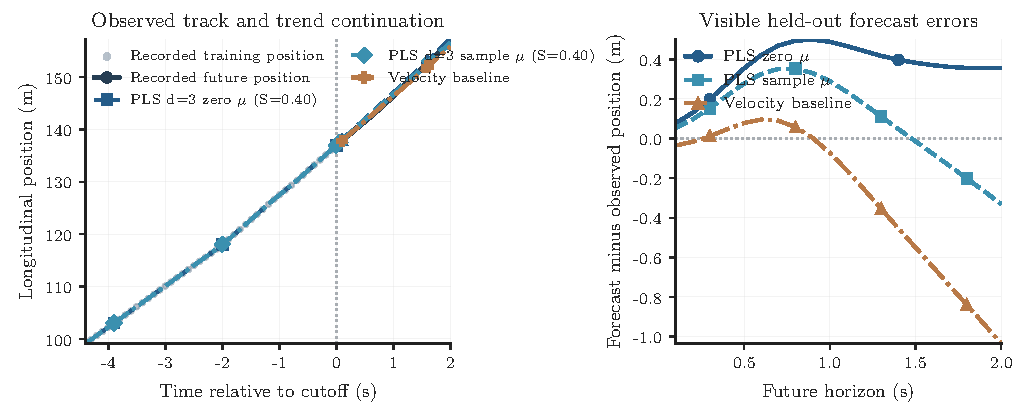
\includegraphics[width=\textwidth]{figures/heldout_forecast.pdf}
\caption{One predeclared US-101 historical
training cutoff, fitted $d=3$ PLS trend
and local-polynomial position continuation.
Future camera-recorded positions are
withheld until evaluation. This is an
illustrative pilot segment, not an
average over the 200-episode study.}
\label{fig:forecast}
\end{figure*}

\begin{figure*}[t]
\centering
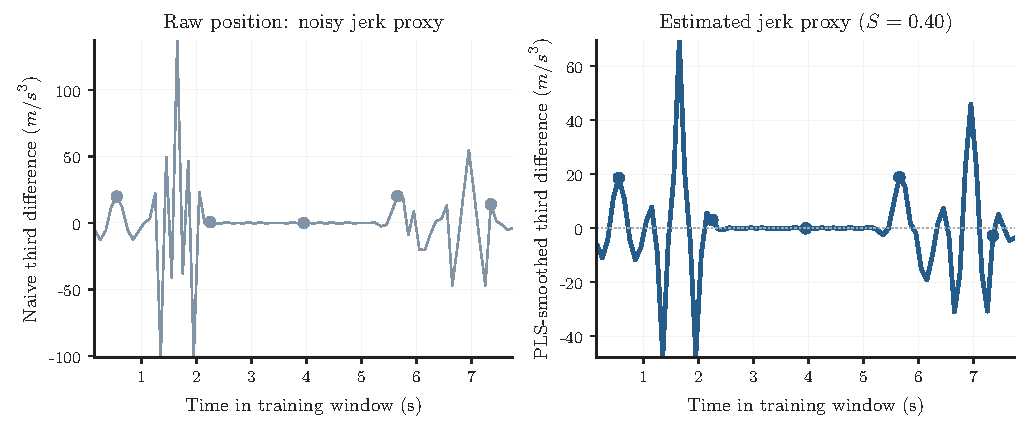
\includegraphics[width=\textwidth]{figures/jerk_comparison.pdf}
\caption{Raw and PLS-smoothed third-difference
\emph{jerk proxies} derived from camera
positions on one US-101 segment. Panel
scales differ and neither plotted
derivative is independently known
to equal the true physical jerk.}
\label{fig:jerk}
\end{figure*}

For the 15-origin pilot the zero-reference
PLS recurrence has the smallest
half-second position RMSE among the
compared variants (0.0745\,m).
The GCV-selected natural cubic spline,
continued by quadratic Taylor expansion,
has the lowest two-second RMSE
(0.8085\,m against 1.2998\,m for the
zero-reference PLS recurrence).
At one second the two are almost tied
(0.2951 versus 0.2958\,m).
The sample-derived nonzero reference
helped the 25-point continuation but
not the last-three-point rule.
These outcomes illustrate
forecast-rule dependence in a
very small set of recorded tracks.

\begin{figure*}[t]
\centering
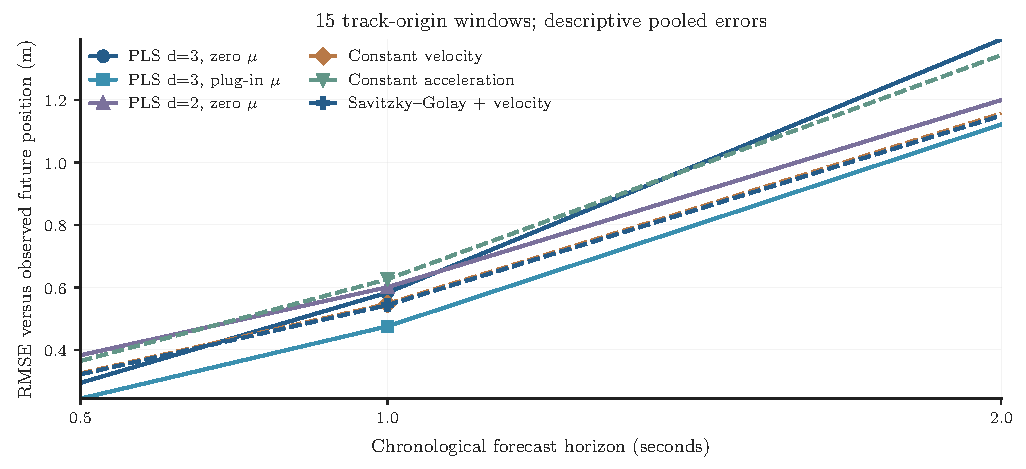
\includegraphics[width=\textwidth]{figures/forecast_horizons.pdf}
\caption{The original exploratory 15-origin
pilot: recorded future-position error
at three horizons for selected PLS
difference orders and conventional
constant-velocity, constant-acceleration
and Savitzky--Golay benchmarks.
Origins overlap within only
five recorded segments.}
\label{fig:horizons}
\end{figure*}

The same pilot compared historical CV,
GCV, AICc, constrained BIC and profile
Gaussian likelihood across difference
orders $d=1,\ldots,4$. Figure
\ref{fig:criteria} visualizes the
resulting criterion-level variation
without treating the five criteria as
independent evidence. The full
pilot tables and forecast rows remain
in the original archive.

\begin{figure*}[t]
\centering
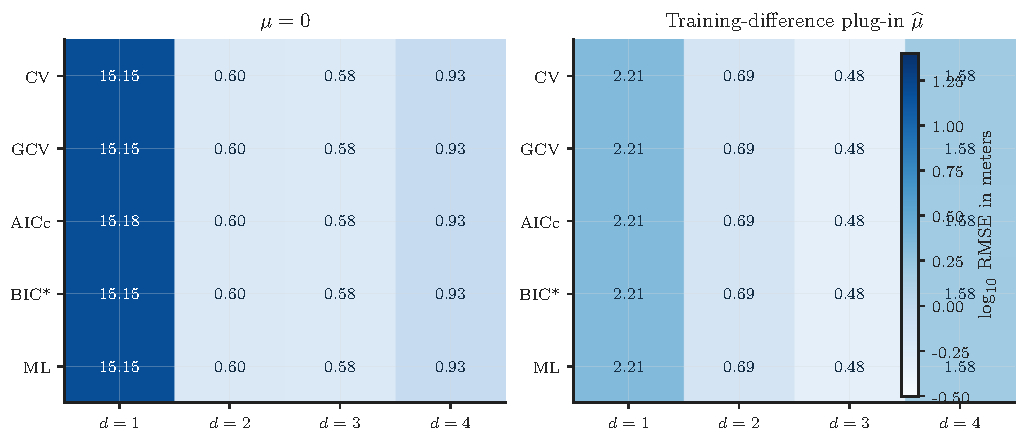
\includegraphics[width=\textwidth]{figures/criterion_heatmap.pdf}
\caption{Exploratory one-second
recorded-position RMSE on the
five-segment pilot, varying PLS
difference order, smoothing criterion
and training-only reference mean.
Colors encode log-RMSE; restricted BIC
uses its documented $S\ge0.10$ bound.
This is a descriptive model
comparison, not a numerical solver
benchmark or significance test.}
\label{fig:criteria}
\end{figure*}
